\section{Secure classical message transmission}
\label{sec:smt}

One of the main tasks in cryptography is to securely transmit a confidential message from one player to another. \emph{Securely} transmitting the message means that the adversary does not learn anything about the message \--- except unavoidable leaks such as the message length \--- and cannot modify the message either. 
% Essentially, what one wishes to
% construct is a secure channel as illustrated in
% \figref{fig:otp.ideal.resource} \--- though, in practice, the
% constructed channel is necessarily weaker, since Eve has the
% possibility of preventing a message from arriving.
We also want to achieve this with minimal assumptions on the available resources. In \figref{fig:construction} we depict the steps necessary to construct such a secure channel from nothing but insecure channels and an initial short key. The aim of this section is to explain this construction in detail. 

In \secref{sec:smt.auth} we first show how to construct an authentic
channel, which is used both by QKD and the OTP. Then in
\secref{sec:smt.qkd} and \secref{sec:smt.otp} we revisit the notions
of a secure key and secure channel resources introduced earlier, and
discuss a modification used here.\footnote{We take into account that
  Eve may prevent the honest players from obtaining the key or the
  transmitted message, which was ignored earlier for simplicity.} In
\secref{sec:smt.together} we put the individual parts of the
construction together and show how this gives a construction of a
secure channel from a short secret key and insecure communication
channels only.

\subsection{Authentication}
\label{sec:smt.auth}

The use of an authentic channel is essential for many cryptographic
protocols, including quantum key distribution, as we have seen
earlier. It allows the players Alice and Bob to be sure that they
are communicating with each other, and not with an adversary Eve. The
authentic channel we used in \secref{sec:qkd} \--- e.g.,
\figref{fig:qkd.real} \--- is however idealized: it guarantees that
the recipient always receives the message that was sent. In a
realistic situation, one has to assume that an adversary may jumble or
cut the communication, and prevent messages from arriving. What still
can be constructed is a channel which guarantees that Bob does not
receive a corrupted message. He either receives the correct message
sent by Alice, or an error, which symbolizes an attempt by Eve to
change the message. This can be modeled by giving Eve's idealized
interface two controls: the first provides her with Alice's message,
the second allows her to input one bit which specifies whether Alice's
message should be delivered or whether Bob gets an error instead. We
illustrate this in \figref{fig:auth.resource}.

\begin{figure}[tb]
% \subcaptionbox[Authentic channel with
% switch]{\label{fig:auth.resource.switch}A resource that allows Eve to
%   decide if Bob gets Alice's message or not, but does not allow the
%   message to be manipulated.}[\columnwidth][c]{
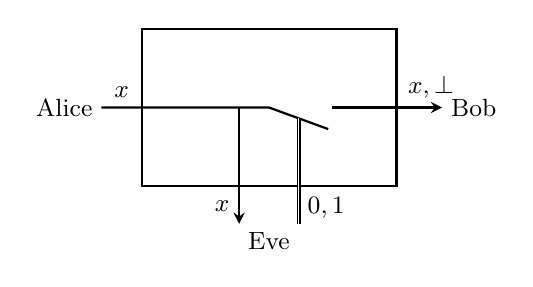
\begin{tikzpicture}[
sArrow/.style={->,>=stealth,thick},
largeResource/.style={draw,thick,minimum width=1.618*2cm,minimum height=2cm}]

\small

\node[largeResource] (keyBox) at (0,0) {};
\node (alice) at (-2.6,0) {Alice};
\node (bob) at (2.6,0) {Bob};
\node (eve) at (0,-1.7) {Eve};
\node (ajunc) at (eve.north west |- alice) {};

\draw[thick] (alice) to node[pos=.12,auto] {$x$} (0,0) to node[pos=.5]
(ejunc) {} +(160:-.8);
\draw[sArrow] (ajunc.center) to node[pos=.85,auto,swap] {$x$} (eve.north west);
\draw[sArrow] (.8,0) to node[pos=.9,auto] {$x,\bot$} (bob);
\draw[double] (ejunc.center |- eve.north) to node[pos=.15,auto,swap] {$0,1$} (ejunc.center);

\end{tikzpicture}
% }

\vspace{6pt}

% \subcaptionbox[Authentic channel with
% two switches]{\label{fig:auth.resource.2switch}If Eve prevents the
%   players from getting a key, then Alice will not even start the
%   protocol, so the constructed ideal resource must have an extra
%   switch to capture this.}[\columnwidth][c]{
% \begin{tikzpicture}[
% sArrow/.style={->,>=stealth,thick},
% largeResource/.style={draw,thick,minimum width=1.618*2cm,minimum height=2cm}]

% \small

% \def\z{.4}

% \node[largeResource] (keyBox) at (0,0) {};
% \node (alice) at (-2.6,0) {Alice};
% \node (bob) at (2.6,0) {Bob};
% \node (eve) at (0,-1.7) {Eve};
% \node (juncLL) at (-3*\z,0) {};
% \node (juncLR) at (-\z,0) {};
% \node (juncRL) at (\z,0) {};
% \node (juncRR) at (3*\z,0) {};

% \draw[thick] (alice) to node[pos=.25,auto] {$x$} (juncLL.center) to node[pos=.5]
% (handle1) {} +(340:2*\z);
% \draw[thick] (juncLR.center) to (juncRL.center) to node[pos=.5]
% (handle2) {} +(340:2*\z);
% \draw[sArrow] (juncRR) to node[pos=.85,auto] {$x,\bot$} (bob);
% \draw[sArrow] (0,0) to node[pos=.85,auto] {$x$} (eve);
% \draw[double] (handle1.center |- eve.north) to node[pos=.15,auto,swap] {$0,1$} (handle1.center);
% \draw[double] (handle2.center |- eve.north) to node[pos=.15,auto,swap] {$0,1$} (handle2.center);

% \end{tikzpicture}
% }
\caption[Authentic channel resource]{\label{fig:auth.resource}An
  authentic channel resource. The message input at Alice's interface
  is visible to Eve, who gets to decide if Bob receives it or not. But
  it guarantees that, if Bob does receive a message, then it
  corresponds to the one sent by Alice.}
\end{figure}

As we are going to explain, such an authentic channel can be
constructed from a completely insecure channel together with a shared
secret key. Although this may be done using a non\-/uniform secret key
[see \textcite{RW03,DW09,ACLV19}], we review here a simpler
construction, originally proposed by \textcite{WC81}, which still only
needs a short key, but which however has to be (close to) uniform: one
computes a hash $h_k(x)$ of the message $x$, and sends the string
$x \| h_k(x)$ to Bob, where $k$ is the short shared secret key and
$\{h_k\}_{k \in \cK}$ a family of strongly universal hash
functions.\footnote{See the formal definition later in this work in
  \footnoteref{fn:universalhash}.} Alice's part of the authentication
protocol $\pi^{\auth}_A$ thus gets as input a key $k$ from an ideal
key resource as well as a message $x$ from Alice, and sends
$x \| h_k(x)$ over the insecure channel. When Bob receives a string
$x' \| y'$, he needs to check whether $y' = h_k(x')$. His part of the
protocol hence gets as input the key $k$ from the ideal key resource,
the message $x' \| y'$ delivered by the channel, and outputs $x'$ if
$y' = h_k(x')$, and otherwise a symbol $\bot$ to indicate an
error. This is depicted in \figref{fig:auth.real}.

\begin{figure}[tb]


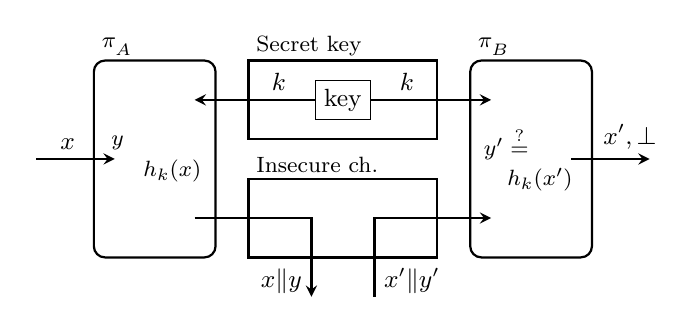
\begin{tikzpicture}[
sArrow/.style={->,>=stealth,thick},
thinResource/.style={draw,thick,minimum width=2.4cm,minimum height=1cm},
protocol/.style={draw,rounded corners,thick,minimum width=1.545cm,minimum height=2.5cm},
pnode/.style={minimum width=1cm,minimum height=.5cm}]

\small

\def\t{3.895} %.75+1.545+.4+1.2
\def\u{2.39} %1.545/2+.4+1.2
\def\v{.75}

\node[pnode] (a1) at (-\u,\v) {};
\node[pnode] (a2) at (-\u,0) {};
\node[pnode] (a3) at (-\u,-\v) {};
\node[protocol,text width=1.1cm] (a) at (-\u,0) {\footnotesize $y
  \coloneqq $\\$\quad \ h_k(x)$};
\node[yshift=-2,above right] at (a.north west) {\footnotesize
  $\pi^{\auth}_A$};
\node (alice) at (-\t,0) {};

\node[pnode] (b1) at (\u,\v) {};
\node[pnode] (b2) at (\u,0) {};
\node[pnode] (b3) at (\u,-\v) {};
\node[protocol,text width=1.2cm] (b) at (\u,0) {\footnotesize $y' \stackrel{?}{=}$\\$\quad h_k(x')$};
\node[yshift=-2,above right] at (b.north west) {\footnotesize $\pi^{\auth}_B$};
\node (bob) at (\t,0) {};

\node[thinResource] (keyBox) at (0,\v) {};
\node[draw] (key) at (0,\v) {key};
\node[yshift=-2,above right] at (keyBox.north west) {\footnotesize
  Secret key $\aK$};
\node[thinResource] (channel) at (0,-\v) {};
\node[yshift=-1.5,above right] at (channel.north west) {\footnotesize
  Insecure ch.~$\aC$};
\node (eveleft) at (-.4,-1.75) {};
\node (everight) at (.4,-1.75) {};
\node (ajunc) at (eveleft |- a3) {};
\node (bjunc) at (everight |- b3) {};

\draw[sArrow] (key) to node[auto,swap,pos=.3] {$k$} (a1);
\draw[sArrow] (key) to node[auto,pos=.3] {$k$} (b1);

\draw[sArrow] (alice.center) to  node[auto,pos=.4] {$x$} (a2);
\draw[sArrow] (b2) to node[auto,pos=.75] {$x',\bot$} (bob.center);

\draw[sArrow] (a3) to (ajunc.center)
to node[pos=.8,auto,swap] {$x \| y$} (eveleft.center);
\draw[sArrow] (everight.center) to node[pos=.2,auto,swap] {$x' \| y'$}
(bjunc.center) to (b3);


\end{tikzpicture}


\caption[Real authentication system]{\label{fig:auth.real}The real
  authentication system consists of the authentication protocol
  $(\pi^{\auth}_A,\pi^{\auth}_B)$ as well as the secret key and insecure
  channel resources, $\aK$ and $\aC$. As in previous illustrations,
  Alice has access to the left interface, Bob to the right interface
  and Eve to the lower interface.}
\end{figure}

To capture completeness of this protocol, one considers instead of the insecure channel $\aC$ as in
\figref{fig:auth.real} a noiseless channel with a
blank interface for Eve\footnote{Unlike in the case of QKD, we do not
  consider noisy channels between Alice and Bob, as such noise could
  be removed easily by encoding the communication with an appropriate classical error
  correcting code. Therefore, the assumed and constructed channels
  faithfully deliver the message from Alice to Bob.}  [as illustrated
in \figref{fig:security.channel.noiseless}], and the constructed
channel is also a perfect noiseless channel instead of the channel
from \figref{fig:auth.resource}. These real and ideal systems are
indistinguishable as they are both identity channels which faithfully
transmit $x$ from Alice to Bob. This proves completeness, and we can therefore focus in the
following on the other part, namely proving soundness of the protocol.

In the ideal setting, the authentic channel
(\figref{fig:auth.resource}) has the same interface on Alice's and
Bob's sides as the real setting (\figref{fig:auth.real}): Alice can
input a message, and Bob receives either a message or an
error. However, Eve's interface looks quite different: in the real
setting she can modify the transmission on the insecure channel,
whereas in the ideal setting the adversarial interface provides only
controls to read the message and interrupt the transmission. From
\defref{def:security} we have that an authentication protocol
constructs the authentic channel if there exists a simulator
$\sigma^{\auth}_E$ that can recreate the real interface while
accessing just the idealized one. An obvious choice for the simulator
is to first generate its own key $k$ and output $x \| h_k(x)$. Then
upon receiving $x' \| y'$, it checks if $x' \| y' = x \| h_k(x)$ and
presses the switch on the authentic channel to output an error if this
does not hold. We illustrate this in \figref{fig:auth.ideal}.

\begin{figure}[tb]


\begin{tikzpicture}[
sArrow/.style={->,>=stealth,thick},
thinResource/.style={draw,thick,minimum width=1.618*2cm,minimum height=1cm},
simulator/.style={draw,rounded corners,thick,minimum width=1.618*2cm,minimum height=1.7cm},
snode/.style={minimum width=1.1cm,minimum height=1.2cm}]

\small

\def\t{2.368} % 1.618+.75
\def\u{-1.1}
\def\v{.75}
\def\w{-2.45} % .25+1.7+.5

\node[thinResource] (channel) at (0,\v) {};
\node[yshift=-1.5,above right] at (channel.north west) {\footnotesize
  Authentic channel $\aA$};
\node (alice) at (-\t,\v) {};
\node (bob) at (\t,\v) {};

\node[simulator] (sim) at (0,\u) {};
\node[xshift=1.5,below left] at (sim.north west) {\footnotesize
  $\sigma^{\auth}_E$};
\node[snode,ellipse] (sleft) at (-.809,\u) {};
\node[snode] (sright) at (.809,\u) {};
\draw[dashed] (sim.north) to (sim.south);

\node (ajunc) at (sleft |- alice) {};
\node (bjunc) at (sright |- bob) {};

\draw[thick] (alice.center) to node[pos=.15,auto] {$x$} (.4,\v) to node[pos=.54] (ejunc) {} +(160:-.8);
\draw[sArrow] (ajunc.center) to node[pos=.63,auto,swap] {$x$} (sleft);
\draw[sArrow] (1.2,\v) to node[pos=.75,auto] {$x,\bot$} (bob.center);
\draw[double] (sright) to node[pos=.4,auto,swap] {$0,1$} (ejunc.center);

\node (sltext) at (-.809,\u) {\footnotesize $y = h_k(x)$};
\node[text width=1.2cm] (srtext) at (.809,\u) {\footnotesize $x \| y
  \stackrel{?}{=}$\\$\quad \ x' \| y'$};

\node (eveleft) at (sleft |- 0,\w) {};
\node (everight) at (sright |- 0,\w) {};
\draw[sArrow] (sleft) to node[pos=.75,auto,swap] {$x \| y$} (eveleft.center);
\draw[sArrow] (everight.center) to node[pos=.25,auto,swap] {$x' \| y'$}
(sright);

\node[draw,fill=white] (key) at (.15,\u+.8) {key};
\draw[sArrow] (key) to (sleft);

\end{tikzpicture}


\caption[Ideal authentication system]{\label{fig:auth.ideal}The ideal authentication system \--- Alice has access to the left interface,  Bob to the right interface and Eve to the lower interface \---  consists of the ideal authentication resource and a simulator  $\sigma^{\auth}_E$.}
\end{figure}

In this case, an authentication protocol is $\eps$\=/secure if Figures~\ref{fig:auth.real} and \ref{fig:auth.ideal} are $\eps$\=/close, i.e.,
\begin{equation} \label{eq:security.auth} \pi^{\auth}_A\pi^{\auth}_B
  \left(\aK \| \aC \right) \close{\eps} \aA\sigma^{\auth}_E.
\end{equation}

Original works defining authentication \--- e.g.,
\textcite{WC81,Sim85,Sim88,Sti90,Sti94} \--- did not use such a
composable security definition. Instead, they considered two kinds of
attacks. In the first, the adversary obtains a pair of a valid message
and authentication tag, and tries to find a pair of a different
message and corresponding valid authentication tag \--- this is called
a \emph{substitution attack}. In the second, the adversary directly
tries to find a pair of message and corresponding valid authentication
tag \--- this is called an \emph{impersonation attack}. It was then
shown that if the family of hash functions used are $\eps$\=/almost
strongly $2$\-/universal,\footnoteremember{fn:universalhash}{A family
  of functions $\{h_k : \cX \to \cY\}_k$ is said to be $\eps$\=/almost
  strongly $2$\-/universal if any two different messages are almost
  uniformly mapped to all pairs of tags, i.e.,
  $\forall x_1,x_2,y_1,y_2,x_1 \neq x_2, \Pr_k \left[ h_k(x_1) = y_1
    \text{ and } h_k(x_2) = y_2\right] \leq
  \frac{\eps}{|\cY|}$~\cite{Sti94}. The family of functions is said to
  be strongly $2$\-/universal if $\eps = 1/|\cY|$.}  the probability
of either of these attacks being successful is bounded by $\eps$. A
composable security proof for these schemes was given by
\textcite{Por14}, who showed that \eqnref{eq:security.auth} is
satisfied, again under the condition that the family of hash functions
used are $\eps$\=/almost strongly
$2$\-/universal.\footnote{\textcite{Por14} additionally shows that
  part of the secret key $k$ can be recycled, since only a number of
  bits corresponding to the length of the hash $h_k(x)$ are
  leaked. This is discussed in \secref{sec:recycle}.}

Note that a distinguisher interacting with either of the real or ideal
systems has the choice between providing messages in two different
orders. It can first provide Alice with a message, receive the
ciphertext\footnote{By \emph{ciphertext} we denote the pair of the
  message and authentication tag generated by the sender.} at Eve's
interface, then input a modified ciphertext, and finally learn whether
the ciphertext is accepted or not at Bob's interface. Or, it can first
input a forged ciphertext at Eve's interface, then learn if it is
accepted, and finally provide Alice with a message and obtain the
corresponding ciphertext at Eve's interface. These two orders of
messages roughly correspond to the substitution and impersonation
attacks.

The secret key resource used so far in this section assumes that both
players always get a copy of the key. However, in \secref{sec:qkd} we
modeled a secret key resource with a switch at Eve's interface, giving
her the possibility to prevent the players from getting the key. If
such a switch is present and Eve flips it, the honest players will not
be able to run the authentication protocol at all. This does however
not change the ideal resource constructed, because not running the
protocol or running the protocol but Eve preventing the message from
being delivered are essentially equivalent. However, the proof in this
case requires a different simulator \--- one which receives the bit
deciding whether the players get a key or not and then acts accordingly.

In \secref{sec:smt.qkd} an even weaker secret key resource is
considered, one which allows Eve to decide if only one of the two
players gets a secret key, but not the other \--- this is drawn in
\figref{fig:key.resource}. Running a similar reasoning as in the
paragraph above, one can see that this does not change the outcome of
the protocol either: it still constructs the authentic channel from
\figref{fig:auth.resource}.

\begin{figure}[tb]

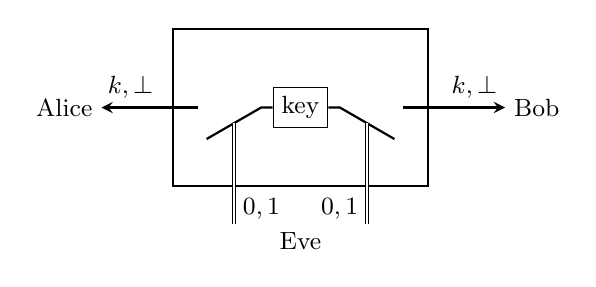
\begin{tikzpicture}[
sArrow/.style={->,>=stealth,thick},
largeResource/.style={draw,thick,minimum width=1.618*2cm,minimum height=2cm}]

\small

\def\u{1.3}
\def\s{.8}

\node[largeResource] (keyBox) at (0,0) {};
\node (alice) at (-3,0) {Alice};
\node (bob) at (3,0) {Bob};
\node (eve) at (0,-1.7) {Eve};
\node[draw] (key) at (0,0) {key};
\node (juncL) at (-\u,0) {};
\node (juncR) at (\u,0) {};

\draw[sArrow] (juncR.center) to node[pos=0.7,auto] {$k,\bot$} (bob);
\draw[sArrow] (juncL.center) to node[pos=0.7,auto,swap] {$k,\bot$} (alice);
\draw[thick] (key) to (-\u+\s,0) to node[pos=.5] (handleL) {} +(210:\s);
\draw[thick] (key) to (\u-\s,0) to node[pos=.5] (handleR) {} +(330:\s);
\draw[double] (handleL |- eve.north) to node[pos=.15,auto,swap] {$0,1$} (handleL.center);
\draw[double] (handleR |- eve.north) to node[pos=.15,auto] {$0,1$} (handleR.center);

\end{tikzpicture}



\caption[Secret key resource with two
switches]{\label{fig:key.resource}A secret key resource allowing Eve
  to control who gets the key: the two bits Eve inputs control whether
  Alice and Bob, respectively, obtain a key or an error message from
  the resource.}
\end{figure}

% The real and ideal systems are trivially identical if
% Eve operates the switch on the left, corresponding to not allowing
% Alice and Bob to generate a key. We can thus in the remainder of this
% section focus on the case is when Eve does not do so, allowing the
% players to run the protocol.

\subsection{Quantum key distribution}
\label{sec:smt.qkd}

In \secref{sec:qkd} we analyzed QKD protocols that use an insecure quantum channel and an authentic channel with the guarantee that the message is always delivered, as indicated in \figref{fig:qkd.real}. The motivation behind this (standard) choice was that, if the message is not delivered, then the players abort and the scheme is trivially secure. In other words, the non-trivial case that needs to be analyzed to prove that a QKD scheme constructs  the ideal key resource is the one in which the adversary does not  use her switch and allows the messages to be delivered on the  authentic channel.

Nonetheless, if we do replace the authentic channel with the one that
can actually be constructed from \figref{fig:auth.resource}, then we
also have to weaken the ideal key resource that is constructed. If the
players get an error message from the authentic channel instead of the
intended message, they will simply abort the protocol and not produce
a key. In the version from \secref{sec:qkd}, Eve already has the power
to prevent the players from getting a secret key. The difference is
that now Eve can let one player get the secret key, but not the other,
e.g., by jumbling the last message between the players. The resulting
ideal key resource is drawn in \figref{fig:key.resource}.

The analysis carried out in \secref{sec:qkd} goes through with only
minor changes with the weaker authentic channel and secret key
resources, since the only differences are the abort conditions, which
now may additionally occur because of failed authentication. In
particular, the reduction from the constructive statement,
\eqnref{eq:qkd.security}, to the trace distance criterion,
\eqnref{eq:qkd.sec}, is unaffected by these changes of resources.

Note that if Eve prevents one player from getting the key, but not the
other, the players are generally unaware of this fact and may end up
with mismatching key lengths.\footnote{The protocol may be designed in
  such a way that the round in which Eve needs to jumble the
  communication so that one player accepts the key but not the other
  is unknown to her. Thus her probability of success will be $O(1/n)$,
  where $n$ is the number of rounds of communication.}  This is not a
problem which is specific to QKD, but happens in general with any key
distribution scheme \cite{Wol99}.

\subsection{One-time pad}
\label{sec:smt.otp}

In \secref{sec:ac.otp} we analyzed the OTP and showed that it
constructs a secure channel given a secret key and an authentic
channel. But again, we used an authentic channel that guarantees that
the message is transmitted, as well as a secret key that is guaranteed
to be delivered to the players. It is however easy to convince oneself
that these extra assumptions about the resources do not affect the
security of the protocol, since if the players do not get a key or a
message they just abort the protocol, in which case security holds
trivially. Therefore, if we plug in the authentic channel from
\figref{fig:auth.resource} and the secret key resource from
\figref{fig:key.resource}, we merely need to weaken the secure channel
that is constructed, so that it may abort as well. We can model this
by adding a switch at Eve's interface that when pressed, delivers an
error message at Bob's interface instead of Alice's message, as
depicted in \figref{fig:secure.resource}. This is very similar to the
authentic channel resource from \figref{fig:auth.resource}, except
that Eve receives only the length of the message rather than the
message itself.

\begin{figure}[tb]

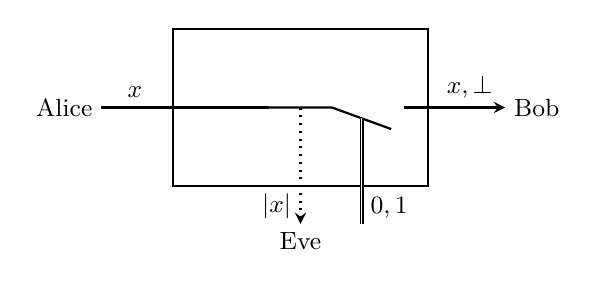
\begin{tikzpicture}[
sArrow/.style={->,>=stealth,thick},
largeResource/.style={draw,thick,minimum width=1.618*2cm,minimum height=2cm}]

\small

\def\z{.4}

\node[largeResource] (keyBox) at (0,0) {};
\node (alice) at (-3,0) {Alice};
\node (bob) at (3,0) {Bob};
\node (eve) at (0,-1.7) {Eve};
\node (juncLL) at (-3*\z,0) {};
\node (juncLR) at (-\z,0) {};
\node (juncRL) at (\z,0) {};
\node (juncRR) at (3*\z,0) {};

% \draw[thick] (alice) to node[pos=.35,auto] {$x$} (juncLL.center) to node[pos=.5]
% (handle1) {} +(340:2*\z);
\draw[thick] (alice) to node[pos=.2,auto] {$x$} (juncLR.center);
\draw[thick] (juncLR.center) to (juncRL.center) to node[pos=.5]
(handle2) {} +(340:2*\z);
\draw[sArrow] (juncRR) to node[pos=.65,auto] {$x,\bot$} (bob);
\draw[sArrow,dotted] (0,0) to node[pos=.85,auto,swap] {$|x|$} (eve);
% \draw[double] (handle1.center |- eve.north) to node[pos=.15,auto,swap] {$0,1$} (handle1.center);
\draw[double] (handle2.center |- eve.north) to node[pos=.15,auto,swap] {$0,1$} (handle2.center);

\end{tikzpicture}



\caption[Secure channel with a switch]{\label{fig:secure.resource}A
  secure channel that allows Eve to learn the length of the message
  and prevent Bob from receiving it: when Alice inputs a message $x$
  at her interface, information about the length of the message is
  given to Eve, who can additionally press a switch that either delivers
  Alice's message to Bob or provides him with an error message $\bot$
  instead.}
\end{figure}

The analysis of the OTP with these altered resources is identical to
the one of \secref{sec:ac.otp}, since the only difference is that both
the real and ideal systems might abort or output an error at Bob's
interface instead of a message if Eve operates the corresponding
switch at her interface.


\subsection{Combining the subprotocols}
\label{sec:smt.together}

Let $\aA$ denote an authentic channel resource, as illustrated in
\figref{fig:auth.resource}, and let $\aK^{\ell}$ denote a secret key
resource of length $\ell$, as drawn in
\figref{fig:key.resource}. Furthermore, let $\aC$ be an insecure
classical, and $\aQ$ an insecure quantum channel. Finally, we denote by $\aS$ a secure classical channel, as depicted in
\figref{fig:secure.resource}. If we summarize the results presented so
far, we have that an authentication protocol constructs an authentic
channel from an insecure channel and a secret key, i.e.,
\[ 
\aK^{a} \| \aC \xrightarrow{\pi^\auth_{AB},\eps_\auth}
\aA;\
\]
a QKD protocol constructs a shared secret key resource from an authentic channel and an insecure quantum channel, i.e., 
\[ 
\aA \| \aQ \xrightarrow{\pi^\qkd_{AB},\eps_\qkd}
\aK^n;\]
and a OTP constructs a secure channel from an authentic channel and a secret key, i.e., 
\[
 \aA \| \aK^m \xrightarrow{\pi^\otp_{AB},0} \aS.
\]
Using also the fact that a key can be split, i.e.,  
\[ 
  \aK^{a+b} \xrightarrow{\id,0} \aK^{a} \| \aK^b ,
  \]
denoting by $a_\qkd$ the length of the key used by the authentication subroutines for QKD,\footnote{A QKD protocol usually authenticates   many messages, which may be going in both directions between Alice and Bob. For   simplicity, we write this here as just one round of authentication, which uses a key of length $a_\qkd$ and has error   $\eps^\qkd_\auth$.} and by $a_\otp$ the length of the key used to authenticate the message for constructing the secure channel, we obtain
\[ 
\aC \| \aC \| \aQ \| \aK^{a_\qkd} \xrightarrow{\pi_{AB},\eps} \aS
\| \aK^{n-m-a_\otp} ,
\]
where $\pi_{AB}$ is the composition of all the protocols and $\eps = \eps_\qkd + \eps_\auth^\qkd + \eps_\auth^\otp$ is the sum of the errors of the individual protocols. We depict this in \figref{fig:secure.complete}, where for simplicity we have drawn only one round of authentication as a subroutine of QKD.

\begin{figure*}[tb]


\begin{tikzpicture}[
resource/.style={draw,thick,minimum width=3cm,minimum height=1cm},
sArrow/.style={->,>=stealth,thick},
sLine/.style={-,thick},
protocol2/.style={draw,thick,minimum width=.6cm,minimum height=2.8cm,rounded corners},
protocol3/.style={draw,thick,minimum width=.6cm,minimum height=4.6cm,rounded corners}]

\small

\def\v{1.8}
\def\x{.5} %1.5/3
\def\p{2.4} % end of resource 1.5 +.6+.6/2
\def\c{1.2} %.6+.6, space between converters
\def\t{7.3}
%\def\z{1.1} %1/2+.6

\node[resource,red] (keyLong) at (0,3*\v) {};
\node[yshift=-1.5,above right] at (keyLong.north west) {\footnotesize
  Secret key $\aK^{a_\qkd}$};
\node[resource,red] (ch1) at (0,2*\v) {};
\node[yshift=-1.5,above] at (ch1.north) {\footnotesize
  Insecure class.\ ch.\ $\aC$};
\node[resource,violet] (chQ) at (0,\v) {};
\node[yshift=-1.5,above] at (chQ.north) {\footnotesize
  Insecure quant.\ ch.\ $\aQ$};
\node[resource,blue] (ch2) at (0,0) {};
\node[yshift=-1.5,above] at (ch2.north) {\footnotesize
  Insecure class.\ ch.\ $\aC$};

\node[protocol2,red] (authqkdA) at (-\p,2.5*\v) {};
\node[yshift=-1.5,above] at (authqkdA.north) {\footnotesize $\pi^\auth_A$};
\node[protocol2,red] (authqkdB) at (\p,2.5*\v) {};
\node[yshift=-1.5,above] at (authqkdB.north) {\footnotesize $\pi^\auth_B$};
\node[protocol3,violet] (qkdA) at (-\p-\c,2*\v) {};
\node[yshift=-1.5,above] (labelA) at (qkdA.north) {\footnotesize $\pi^\qkd_A$};
\node[protocol3,violet] (qkdB) at (\p+\c,2*\v) {};
\node[yshift=-1.5,above] (labelB) at (qkdB.north) {\footnotesize $\pi^\qkd_B$};
\node[protocol2,blue] (authotpA) at (-\p-2*\c,\v/2) {};
\node[yshift=-1.5,above] at (authotpA.north) {\footnotesize $\pi^\auth_A$};
\node[protocol2,blue] (authotpB) at (\p+2*\c,\v/2) {};
\node[yshift=-1.5,above] at (authotpB.north) {\footnotesize $\pi^\auth_B$};
\node[protocol3,green] (otpA) at (-\p-3*\c,\v) {};
\node[yshift=-1.5,above] at (otpA.north) {\footnotesize $\pi^\otp_A$};
\node[protocol3,green] (otpB) at (\p+3*\c,\v) {};
\node[yshift=-1.5,above] at (otpB.north) {\footnotesize $\pi^\otp_B$};

\node[draw,thick,dashed,fit=(authqkdA)(labelA)(otpA),inner sep=8] (compA) {};
\node[yshift=-1.5,above right] at (compA.north west) {\footnotesize
  Composed protocol $\pi_A$};
\node[draw,thick,dashed,fit=(authqkdB)(labelB)(otpB),inner sep=8] (compB) {};
\node[yshift=-1.5,above right] at (compB.north west) {\footnotesize
  Composed protocol $\pi_B$};

\node (p1) at (0,5*\v/2) {};
\node (p2) at (0,3*\v/2) {};
\node (p3) at (0,\v/2) {};
\node (p4) at (0,-\v/2) {};
\node (aliceUp) at (-\t,3*\v) {};
\node (aliceDown) at (-\t,\v) {};
\node (bobUp) at (\t,3*\v) {};
\node (bobDown) at (\t,\v) {};

\node (eveLeft) at (-\x,0) {};
\node (eveRight) at (\x,0) {};

\draw[sArrow] (aliceDown.center) to node[auto,pos=.35] {$x$} (otpA.west |- aliceDown);
\draw[sArrow] (otpA.east |- p3) to (authotpA.west |- p3);
\draw[sArrow] (qkdA.west |- aliceUp) to node[auto,pos=.9,swap] {$k_1$} (aliceUp.center);
\draw[sArrow] (qkdA.west |- 0,2*\v) to node[auto,pos=.5,swap] {$k_2$} (otpA.east |- 0,2*\v);
\draw[sArrow] (qkdA.west |- 0,\v) to node[auto,pos=.5,swap] {$k_3$} (authotpA.east |- 0,\v);
\draw[sArrow] (authotpA.east |- 0,0) to (eveLeft |- 0,0) to (eveLeft |- p4);
\draw[sArrow] (qkdA.east |- 0,\v) to (eveLeft |- 0,\v) to (eveLeft |- p3);
\draw[sArrow] (qkdA.east |- p1) to (authqkdA.west |- p1);
\draw[sArrow] (authqkdA.east |- 0,2*\v) to (eveLeft |- 0,2*\v) to (eveLeft |- p2);
\draw[sArrow] (keyLong.west |- 0,3*\v) to (authqkdA.east |- 0,3*\v);

\draw[sArrow] (keyLong.east |- 0,3*\v) to (authqkdB.west |- 0,3*\v);
\draw[sArrow] (eveRight |- p2) to (eveRight |- 0,2*\v) to (authqkdB.west |- 0,2*\v);
\draw[sArrow] (eveRight |- p3) to (eveRight |- 0,\v) to (qkdB.west |- 0,\v);
\draw[sArrow] (eveRight |- p4) to (eveRight |- 0,0) to (authotpB.west |- 0,0);
\draw[sArrow] (authqkdB.east |- p1) to (qkdB.west |- p1);
\draw[sArrow] (qkdB.east |- aliceUp) to node[auto,pos=.9] {$k'_1$} (bobUp.center);
\draw[sArrow] (qkdB.east |- 0,2*\v) to node[auto,pos=.5] {$k'_2$} (otpB.west |- 0,2*\v);
\draw[sArrow] (qkdB.east |- 0,\v) to node[auto,pos=.5] {$k'_3$} (authotpB.west |- 0,\v);
\draw[sArrow] (authotpB.east |- p3) to (otpB.west |- p3);
\draw[sArrow] (otpB.east |- bobDown) to node[auto,pos=.65] {$x'$} (bobDown.center);

\end{tikzpicture}


\caption[Constructing a secure channel]{\label{fig:secure.complete}
  (Color online)
  Composition of QKD, authentication and OTP protocols. For
  simplicity, we have drawn only one round of authentication as a
  subroutine of QKD as \textcolor{red}{$\pi^\auth_{AB}\left(
      \aK^{a_\qkd} \| \aC \right)$}. The \textcolor{violet}{QKD
    protocol $\pi^{\qkd}_{AB}$} constructs a shared key resource that
  produces the long key $(k_1,k_2,k_3)$. The second
  \textcolor{blue}{authentication protocol $\pi^\auth_{AB}$} then uses
  part of this key to construct another authentic channel, and the
  \textcolor{green}{OTP protocol $\pi^{\otp}_{AB}$} uses another part
  of this key to encrypt and decrypt the message sent on the channel.}
\end{figure*}


%%% Local Variables:
%%% TeX-master: "main.tex"
%%% End: